Classic mixture models make the assumption that the data are drawn
from a finite collection of distributions. A data point is generated
by first selecting one of the class distributions, and then drawing a
sample from that distribution. In this model, the $X^n$ are observed
and the cluster indicators $Z^n$, cluster mixture weights $\pi_{1:K}$
and the parameters of the distributions $\theta_{1:K}$ are
hidden. Such models are useful for clustering, since we can infer the
hidden cluster indicators $Z^n$ to recover a partition of the data
that is likely according to the generative story sketched above.

While mixture models are useful and can act as fundamental components
of more sophisticated hierarchical models, it is often difficult in
practice to choose the correct number of clusters $K$ that should be
used. This is known as model selection, and is often done by learning
models for a variety of $K$ and assessing the fit of each model using
a metric such as held-out log likelihood or Akaike information
criterion.

An alternative to model selection is to use Bayesian nonparametric
models such as the Dirichlet process mixture model \cite{antoniak1974}
which assumes \textit{a priori} that there are an infinite number of
clusters (i.e. $K \to \infty$). While theoretically infinite, the
Dirichlet process generates mixture weights $\pi_{1:\infty}$ over the
clusters where finitely many of the clusters have non-zero
probabilities. While there is no known density function for this
distribution, there are several algorithms available that can sample
from the Dirichlet process, which makes this powerful model usable in
practice.

In a mixture model, we are interested in recovering the cluster
indicators $Z^n$. An equivalent formulation of the cluster indicators
$Z^n$ is to recover a partition of the data $X^n$. The Chinese
Restaurant Process (CRP) is an algorithm for sampling partitions of a
dataset from a DP in which the random measure that we sample from the
DP has been integrated out.

\begin{figure}[h]
\centering
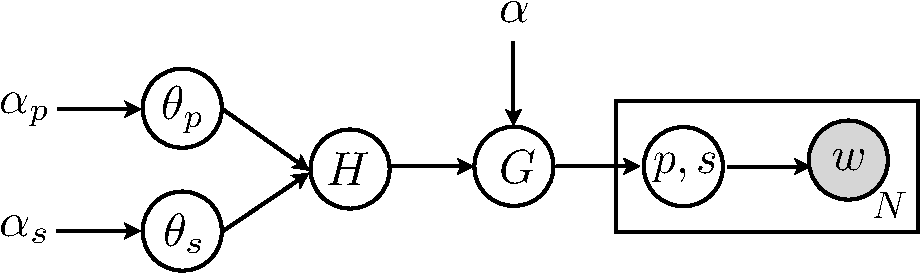
\includegraphics[width=0.9\textwidth]{fig/v2}
\caption{Reparametrized model}
\label{fig:v1}
\end{figure}

\begin{align*}
\theta_p & \sim \text{Dir}(\alpha_p) \\
\theta_s & \sim \text{Dir}(\alpha_s) \\
H(p, s) & = p(p \mid \theta_p) p(s \mid \theta_s) \\
G & \sim \text{DP}\left(\alpha, H\right)\\
\forall i \in \{1 \dots N\} \\
(p_i, s_i) & \sim G \\
w_i & = p_i+s_i
\end{align*}
